\subsection{Protocol}\label{PROTOKOL}
Protokollen til systemet blev tidligt besluttet at skulle fungere ved at sende strenge af XML over en socket forbindelse. Da det kom til den reelle udvikling af hvordan denne XML string skulle genereres blev der opsat nogle begreber til videre udarbejdelse:

\begin{itemize}
\item \textbf{Encode} Der skulle kunne gives et forudbestemt data objekt til en encode funktion der herefter skulle sørge for at generere en passende XML string. 
\item \textbf{Decode} Der skulle ligeledes kunne gives en string med XML som en decode funktion herefter kunne danne et passende data objekt udfra. 
\item \textbf{Commands} De kommandoer der skulle videregives informationer om skulle fungere som objekter der på bagrund af informationen i dem, kunne handles på andetsteds.
\item \textbf{Marshallers} Der skulle ligge noget logik "bagved" protocol objektet, som her skulle sørge for den reelle ændring fra det XML til data og omvendt. Det blev derfor nødvendigt at lave en Marshaller for hver Command som protocol objektet kunne kalde på.
\end{itemize}

For at "legemligøre" denne protocol blev der udarbejdet en protocol klasse. Denne vil på sigt kunne sætte sin egen marshaller attribut, og dermed vælge hvilket sprog der parses om til. Men da der i dette projekt som udgangspunkt kun bruges XML, sættes Protocol klassens marshaller attribut altid til XmlMarshal klassen.

Protocol klassen vil udover kommandoer være det eneste der bliver stiftet bekendtskab med når der skal parses. Udviklere vil på den måde ikke skulle rode med marshallers og interfaces længere nede i lagene og på den måde kan alt funktionalitet omkring systemets protokol forholdsvis simpelt tilgås fra et højere abstraktionsniveau.

\begin{figure}[H]
	\centering
	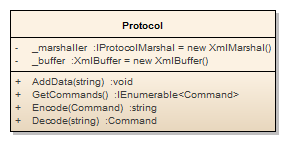
\includegraphics[width=0.6\textwidth]{Systemdesign/SharedLib/Images/Klasser/Protocol.png}
	\caption{Protocol klassen}
	\label{fig:klasseProtocol}
\end{figure}


\begin{figure}[H]
    \centering
    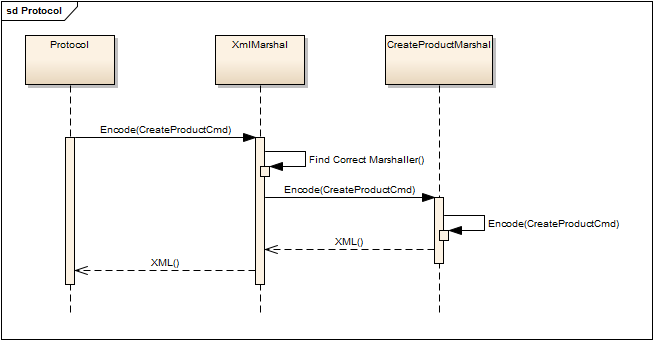
\includegraphics[width=1.0\textwidth]{Systemdesign/SharedLib/Images/Protokol/Protocol_Sek.png}
    \caption{Sekvensdiagram over protokollens encode funktion}
    \label{fig:protocolSek}
\end{figure}

På figur \ref{fig:protocolSek} er der illustreret et scenarie hvor der bliver kaldt Encode med en CreateProduct kommando på protocol objektet, dette kan f.eks. være \gls{AS} der vil oprette et produkt i databasen og derfor skal sende denne besked over socket forbindelsen.

\gls{AS} vil derfor lave en instans af den givne kommando klasse, en instans af protocol klassen. Herefter kaldes Encode fra protocol objektet med kommandoen og denne vil herefter kalde Encode med kommandoen på den korrekte marshaller, som til sidst reelt parser objektet om til en XML string og sender dette tilbage gennem XmlMarshal klassen og tilbage til protocol objektet. 

Som det ses på figur \ref{fig:protocolSek}, er der ikke mange kald der bliver lavet når en kommando bliver parset, Dog sker der en masse logik i de enkelte klasser. Da protocol klassen blev udarbejdet blev det besluttet at der skulle være mulighed for udvidelse af systemet så der kunne sendes med andre dataformater end XML over socket forbindelserne. derfor blev der oprette et interface til XmlMarshal klassen som denne implementere og dette er derfor det første protocol tager stilling til.

Derefter er der et hav af commands og marshallers, og for at følge Open-Closed princippet skulle det på sigt være muligt at kunne sende andre commandoer over systemet. Derfor tager XmlMarshal stilling til, på baggrund af den indkomne kommandos navn, hvilken Marshaller der er passende for denne kommando og kalder, hvis denne eksisterer, encode/decode på denne marshaller.